%% Comparative Evaluation of Unsupervised Machine Learning Models for
%% Multivariate Sensor Anomaly Detection in Industrial Systems
%%
%% IEEE Conference template (IEEEtran). Compile with pdflatex:
%%   pdflatex paper.tex   (run twice so references/labels resolve)
%%
%% Figures are read from ../results/figures/ (generated by `python main.py`).

\documentclass[conference]{IEEEtran}
\IEEEoverridecommandlockouts

\usepackage{cite}
\usepackage{amsmath,amssymb,amsfonts}
\usepackage{graphicx}
\usepackage{booktabs}
\usepackage{textcomp}
\usepackage{xcolor}
\usepackage{url}

% Figures live alongside the generated results.
\graphicspath{{../results/figures/}}

\begin{document}

\title{Comparative Evaluation of Unsupervised Machine\\ Learning Models for Multivariate Sensor Anomaly\\ Detection in Industrial Systems}

\author{
\IEEEauthorblockN{Sarjan Shah}
\IEEEauthorblockA{\textit{Department of Information Technology} \\
\textit{[Institution]}\\
[City, Country] \\
neesheshah@gmail.com}
\and
\IEEEauthorblockN{Abhi Shah}
\IEEEauthorblockA{\textit{Department of Information Technology} \\
\textit{[Institution]}\\
[City, Country] \\
[email]}
}

\maketitle

\begin{abstract}
Industrial machinery is increasingly instrumented with multiple sensors whose
readings can reveal incipient faults, yet labelled fault data is rarely
available in practice, motivating \emph{unsupervised} anomaly detection that
learns only from normal operation. This paper presents a controlled,
reproducible comparison of six unsupervised anomaly-detection models---a
statistical $z$-score baseline, One-Class SVM, Local Outlier Factor (LOF),
Principal Component Analysis (PCA) reconstruction error, the Elliptic Envelope
(robust covariance), and Isolation Forest---on the Skoltech Anomaly Benchmark
(SKAB), a real multivariate sensor dataset from a water-circulation testbed
with induced valve faults. All models are trained on an identical, leakage-free
feature representation and evaluated on a strictly held-out, chronologically
separated test set, so that differences in score reflect the models rather than
the experimental setup. Isolation Forest achieves the best overall performance
(F1 $=0.466$, recall $=0.656$), outperforming every other method including the
two correlation-based models that are theoretically expected to exploit
inter-sensor structure. We report results honestly, including the modest
absolute precision typical of real industrial benchmarks, and we document a
wall-clock feature leak that we identified and removed. The study contributes a
transparent baseline and a methodological template for evaluating unsupervised
detectors on real sensor data.
\end{abstract}

\begin{IEEEkeywords}
anomaly detection, unsupervised learning, multivariate time series, industrial
sensors, predictive maintenance, Isolation Forest, SKAB
\end{IEEEkeywords}

\section{Introduction}
Modern industrial systems---pumps, motors, valves, and the pipework that
connects them---are routinely instrumented with sensors measuring vibration,
pressure, temperature, current, and flow. These signals carry early evidence of
developing faults, and detecting that evidence before failure is the goal of
condition monitoring and predictive maintenance, where machine-learning methods
have become central~\cite{rotating2023}. The dominant practical difficulty is
that \emph{labelled} fault data is scarce: faults are rare, diverse, and
expensive to induce or annotate, so a supervised classifier trained to
recognise specific known faults generalises poorly to the next, unseen
failure mode~\cite{chandola2009}.

Unsupervised anomaly detection sidesteps this problem. Rather than learning to
separate ``normal'' from labelled ``fault'' examples, an unsupervised
(or \emph{novelty}) detector is trained only on data representing healthy
operation; at inference time it flags any reading that deviates sufficiently
from the learned notion of normal. This framing matches the reality of
industrial deployment, where abundant normal data is available but fault labels
are not~\cite{belay2023}.

A large and growing toolbox of unsupervised detectors exists, ranging from
simple statistical thresholds to deep reconstruction
networks~\cite{chalapathy2019}. For a practitioner, the relevant question is not
``what is the most sophisticated method?'' but ``which method actually performs
best on real sensor data, under a fair and honest evaluation?'' Surprisingly,
this question is often answered on synthetic data, with optimistic evaluation
protocols, or without controlling for information leakage---all of which inflate
reported scores.

This paper makes the following contributions:
\begin{itemize}
\item We conduct a controlled comparison of \textbf{six} classical unsupervised
anomaly-detection models on the \textbf{real} Skoltech Anomaly Benchmark (SKAB),
using a single shared feature representation so that the comparison isolates the
detector rather than the preprocessing.
\item We adopt a deliberately conservative evaluation protocol: a
\emph{chronological}, per-experiment train/test split with no shuffling, an
unsupervised training set kept free of labelled anomalies, and validation-based
hyperparameter selection that we audit for degenerate ``flag-everything''
behaviour.
\item We identify and remove a \emph{data leak} caused by wall-clock features,
and report the resulting (lower but trustworthy) scores, providing a transparent
account of how methodological rigour affects the headline number.
\item We find that \textbf{Isolation Forest} is the strongest detector on this
benchmark, and we analyse why two theoretically higher-ranked correlation-based
models do not surpass it on engineered tabular features.
\end{itemize}

The remainder of the paper is organised as follows. Section~\ref{sec:related}
reviews related work. Section~\ref{sec:dataset} describes the SKAB dataset.
Section~\ref{sec:method} details the feature engineering, the six models, and
the evaluation protocol. Section~\ref{sec:results} presents the results.
Section~\ref{sec:discussion} discusses findings and limitations, and
Section~\ref{sec:conclusion} concludes.

\section{Related Work}
\label{sec:related}
Anomaly detection is a mature field with a well-established taxonomy of
statistical, distance-based, density-based, and classification-based
approaches~\cite{chandola2009}. Classical methods remain widely used because
they are fast, interpretable, and require little tuning. Distance- and
density-based detectors such as the Local Outlier Factor (LOF) score a point by
the relative density of its local neighbourhood~\cite{breunig2000}, while
boundary methods such as the One-Class SVM learn a decision surface enclosing
the bulk of the normal data~\cite{scholkopf2001}. Covariance-based methods
model the normal data as a single distribution and flag points with large
Mahalanobis distance; the Elliptic Envelope uses the robust Minimum Covariance
Determinant estimator to make this estimate resistant to
contamination~\cite{rousseeuw1999}. Reconstruction-based detectors, of which PCA
reconstruction error is the linear archetype, project data onto a low-rank
normal subspace and flag points that reconstruct poorly~\cite{shyu2003}.
Isolation Forest takes a different route, isolating anomalies directly through
random recursive partitioning under the premise that anomalies are ``few and
different'' and therefore easier to isolate~\cite{liu2008}.

More recently, deep learning has been applied extensively to anomaly
detection~\cite{chalapathy2019}. Sequence models such as LSTM-based
encoder--decoders learn to reconstruct normal multivariate sensor sequences and
use reconstruction error as the anomaly score~\cite{malhotra2016}. Such models
can capture temporal dependencies that tabular methods do not, but they require
substantially more data, compute, and tuning, and recent surveys note that on
many real multivariate-time-series benchmarks they do not consistently dominate
simpler approaches~\cite{belay2023}. Our work is positioned deliberately within
the classical regime: we ask how far well-engineered features plus standard
unsupervised detectors can go on a real benchmark, and we provide an honest
baseline against which heavier models can be compared.

\section{Dataset}
\label{sec:dataset}
We use the Skoltech Anomaly Benchmark (SKAB)~\cite{skab2020}, a publicly
available collection of multivariate sensor time series recorded from an
industrial water-circulation testbed at the Skolkovo Institute of Science and
Technology. The testbed comprises a pump, pipework, and valves, and faults are
induced physically, primarily by partially closing a valve to restrict flow.

Each recording samples eight sensors at 1\,Hz: two accelerometers
(vibration RMS at two mount points), motor current, system pressure, water
temperature, pump-housing thermocouple temperature, supply voltage, and
volumetric flow rate (RMS). The corpus contains 35 CSV files: one
\emph{anomaly-free} baseline run of healthy operation (without label columns),
and 34 fault runs organised into three groups---\texttt{valve1} (16 runs),
\texttt{valve2} (4 runs), and \texttt{other} (14 runs of miscellaneous faults).
Each fault run carries two binary labels per timestamp: \texttt{anomaly}
($1$ during a fault, $0$ otherwise) and \texttt{changepoint} (marking the
instant of transition). Crucially, each CSV is an \emph{independent} experiment
with its own clock; the runs are not a single continuous stream.

In total the fault runs contribute 37{,}459 labelled rows and the baseline run
9{,}401 rows. Across the fault corpus the anomaly rate is high relative to a
typical monitoring setting (faults are sustained for substantial portions of
each run), which we account for in our evaluation by reporting precision,
recall, and F1 rather than accuracy.

\section{Methodology}
\label{sec:method}

\subsection{Feature Engineering}
Raw sensor values alone discard temporal context, so we augment each timestamp
with short-horizon causal statistics. For every sensor we compute, using only
the current and past readings: a 5-second rolling mean, a 5-second rolling
standard deviation, a 30-second rolling mean, and the first difference (delta).
We retain the raw value and add one global feature, \texttt{time\_since\_start}
(elapsed seconds within a run). This yields \textbf{41 features}
($8 \text{ sensors} \times 5 + 1$).

Two design choices guard against contamination of the feature space. First,
all rolling statistics are computed \emph{per experiment}: a window is never
allowed to span the boundary between two independent runs, which would
manufacture a spurious correlation between unrelated physical conditions.
Second, we deliberately \emph{exclude} wall-clock features (hour-of-day,
day-of-week). We initially included them and observed a small score increase,
but an ablation revealed this to be \emph{leakage}: because the test set is the
chronological tail of the same files used for training, within a short run the
hour is near-constant and acts as a hidden identifier for ``which experiment
this is,'' allowing a model to recall a file's fault propensity rather than
detect a physical anomaly. Removing these features lowered the headline F1 but
produced a number that generalises honestly; all results below use the
leakage-free 41-feature representation.

\subsection{Train/Validation/Test Split}
Because the data is a time series, we never shuffle. Each fault file is split
chronologically into the first 80\% (training portion) and the final 20\%
(test portion), and these portions are concatenated across files to form the
global train and test sets. The unsupervised training set is then constructed
to contain \emph{only normal operation}: it combines the entire anomaly-free
baseline run with the \texttt{anomaly}$=0$ rows of each fault file's training
portion. This keeps the training data $100\%$ free of labelled anomalies---the
methodologically correct setting for a novelty detector---while still exposing
the models to the realistic operating diversity of the fault rigs (not only the
single pristine baseline run). The resulting training set contains
\textbf{28{,}368 rows}; the test set contains \textbf{7{,}503 rows}, of which
2{,}252 ($30.0\%$) are anomalous. Hyperparameters are selected on a validation
set held out at the granularity of \emph{whole experiment files} (rather than a
time slice), which avoids a pathological case in which a naive time-based
validation split fell almost entirely inside a sustained-fault block. All
features are standardised with a \texttt{StandardScaler} fit on the training set
only and applied unchanged to the test set.

\subsection{Models}
We evaluate six unsupervised detectors, all from
scikit-learn~\cite{pedregosa2011} except the statistical baseline, behind a
common train/predict interface and on the identical scaled feature matrix:
\begin{itemize}
\item \textbf{$z$-score} (statistical baseline): flags a row if any feature
exceeds a fixed number of standard deviations from the training mean.
\item \textbf{One-Class SVM}~\cite{scholkopf2001}: an RBF-kernel boundary around
the normal data, parameterised by $\nu$.
\item \textbf{Local Outlier Factor}~\cite{breunig2000}, in novelty mode so it
can score held-out points.
\item \textbf{PCA reconstruction error}~\cite{shyu2003}: retain the components
explaining 95\% of training variance; the anomaly score is the residual
reconstruction error.
\item \textbf{Elliptic Envelope}~\cite{rousseeuw1999}: robust Gaussian
(Mahalanobis) modelling via Minimum Covariance Determinant. As the 41 features
are partly collinear (rolling means track raw values), the raw covariance is
singular; we therefore PCA-whiten to 10 decorrelated components before fitting,
a standard numerically stable Mahalanobis setup.
\item \textbf{Isolation Forest}~\cite{liu2008}: an ensemble of random isolation
trees; the anomaly score reflects how shallowly a point is isolated.
\end{itemize}
The contamination parameter (the assumed anomaly fraction) was tuned on the
validation set. Isolation Forest's sweep exhibited a genuine interior optimum at
$0.35$; for consistency this shared assumption was applied across the
contamination/$\nu$-based models. We explicitly rejected validation optima that
corresponded to degenerate ``flag-everything'' behaviour (recall near $100\%$),
which inflate F1 without providing a useful detector.

\subsection{Evaluation Metrics}
We report precision, recall, and F1 on the anomaly (positive) class, together
with the confusion matrix. Precision is the fraction of flagged rows that are
truly anomalous; recall is the fraction of true anomalies that are flagged; F1
is their harmonic mean. We treat F1 as the headline metric because, unlike
accuracy, it is not satisfied by a detector that simply abstains or simply
alarms on everything.

\section{Results}
\label{sec:results}

Table~\ref{tab:results} reports the performance of all six models on the
held-out test set, sorted by F1. Isolation Forest is the best model on every
axis that matters for this task: it attains the highest F1 ($0.466$) and, by a
clear margin, the highest recall ($0.656$), while maintaining precision
comparable to the field. Figure~\ref{fig:comparison} visualises the same
comparison.

\begin{table}[t]
\caption{Test-set performance of the six unsupervised models, sorted by F1.
Best value in each column is in \textbf{bold}.}
\label{tab:results}
\centering
\begin{tabular}{lccc}
\toprule
\textbf{Model} & \textbf{Precision} & \textbf{Recall} & \textbf{F1} \\
\midrule
Isolation Forest          & \textbf{0.362} & \textbf{0.656} & \textbf{0.466} \\
Elliptic Envelope         & 0.342 & 0.539 & 0.418 \\
$z$-score (baseline)      & 0.329 & 0.548 & 0.411 \\
One-Class SVM             & 0.326 & 0.537 & 0.406 \\
Local Outlier Factor      & 0.321 & 0.460 & 0.378 \\
PCA reconstruction        & 0.305 & 0.470 & 0.370 \\
\bottomrule
\end{tabular}
\end{table}

\begin{figure}[t]
\centering
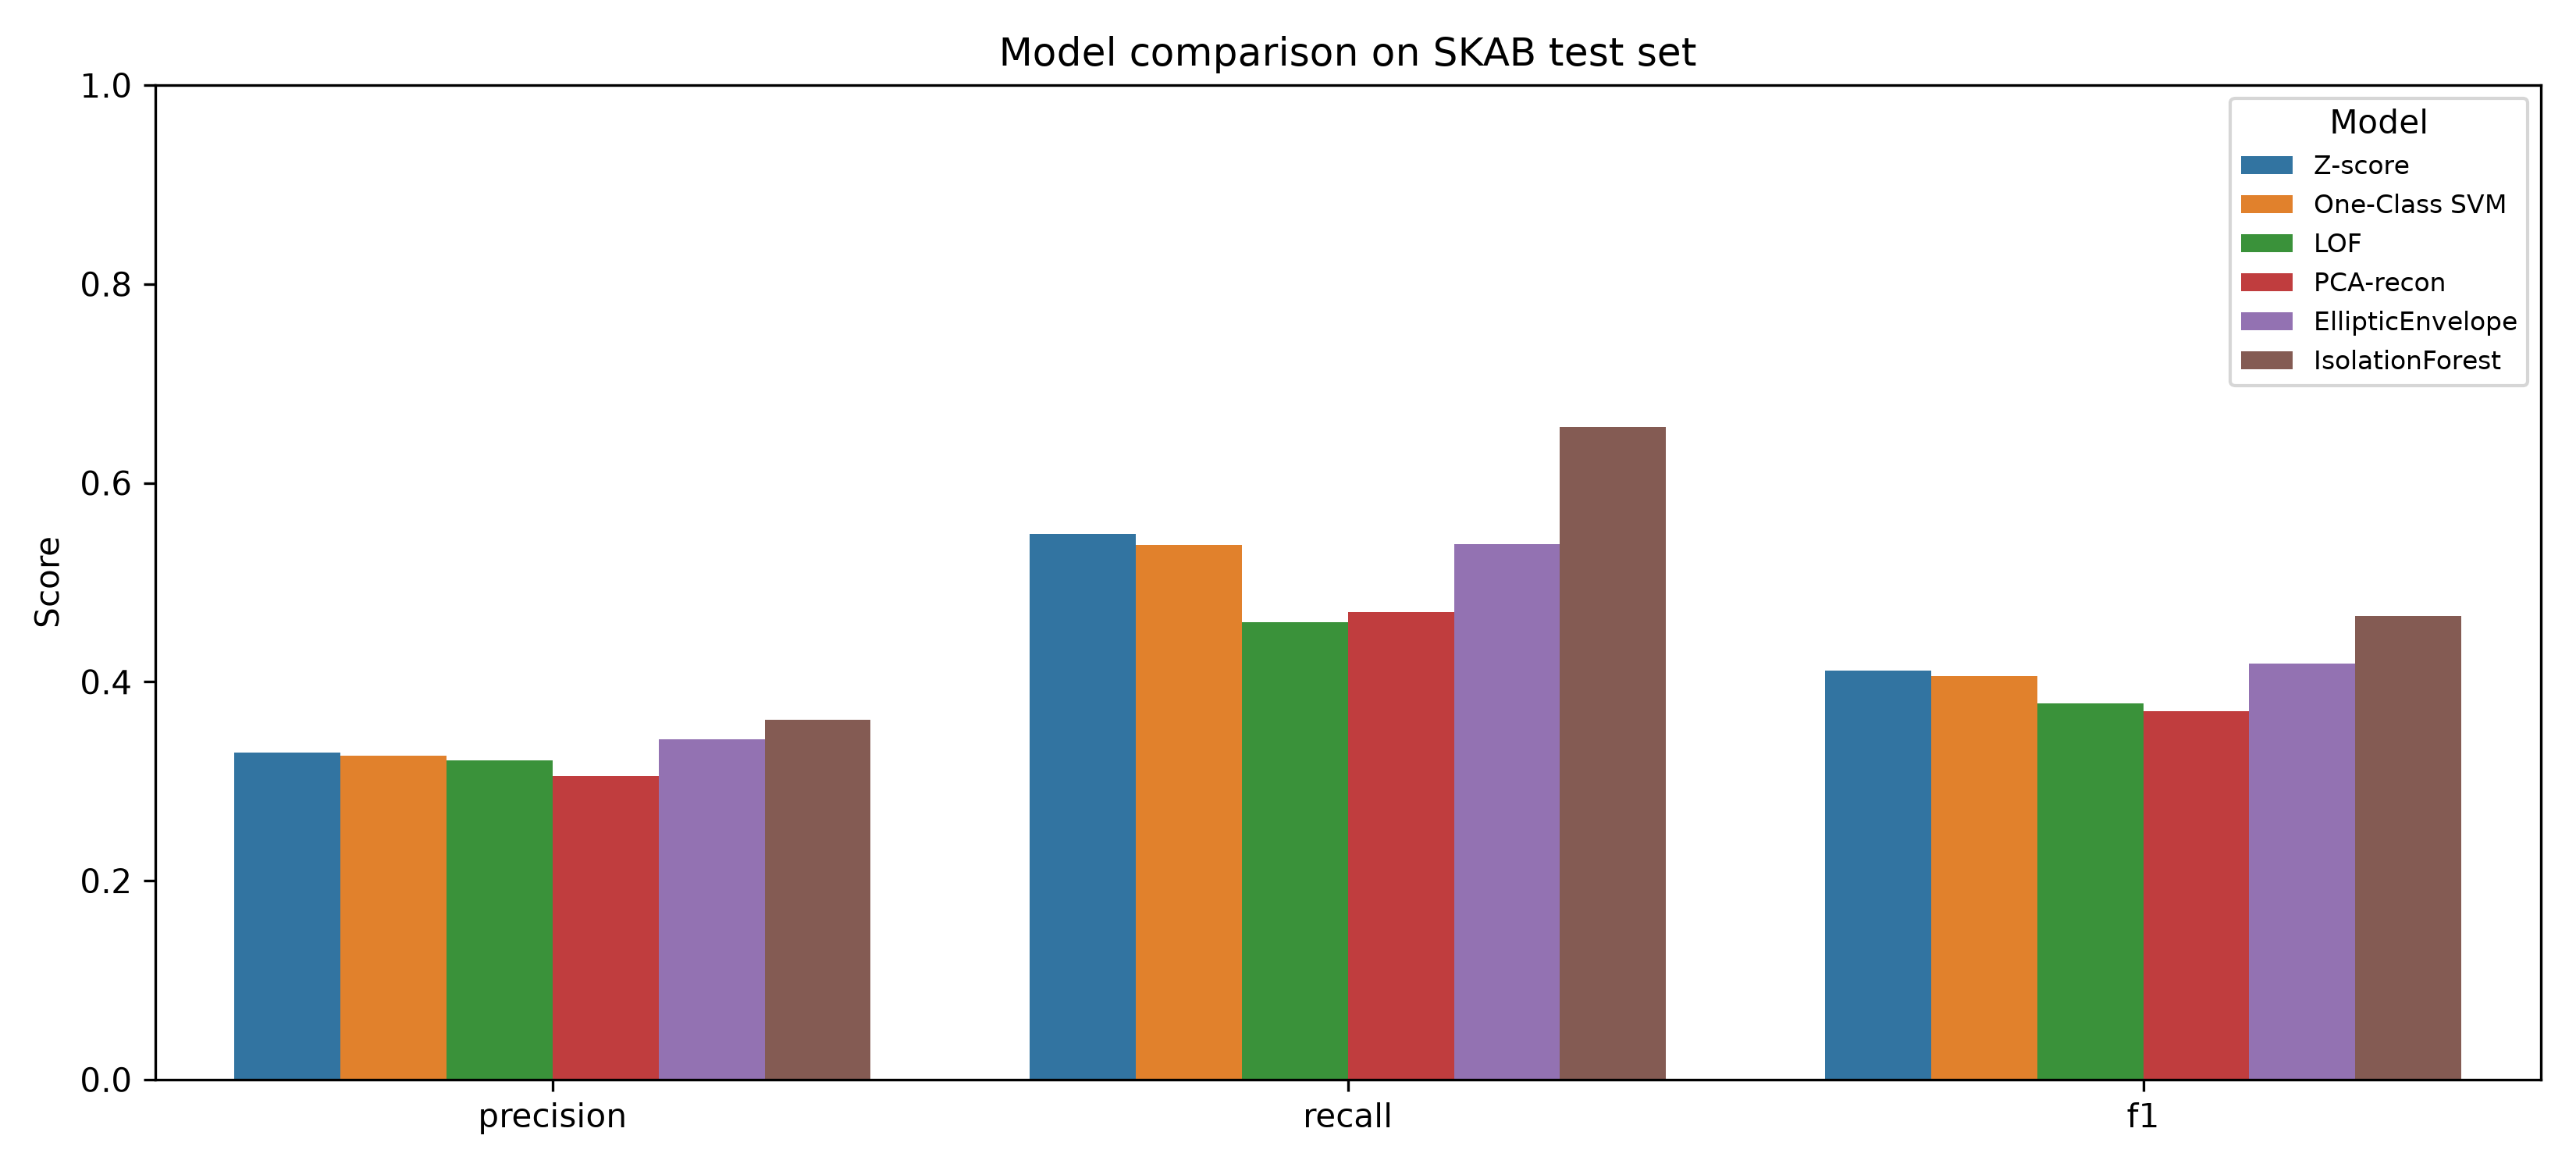
\includegraphics[width=\columnwidth]{model_comparison.png}
\caption{Precision, recall, and F1 for all six models. Isolation Forest (right
bar in each cluster) leads on recall and F1.}
\label{fig:comparison}
\end{figure}

\subsection{Error Analysis}
Figure~\ref{fig:confusion} shows the per-model confusion matrices. Of the
2{,}252 true fault-seconds in the test set, Isolation Forest correctly catches
\textbf{1{,}477} and misses 775, the fullest true-positive count of any model.
It raises 2{,}608 false alarms against 2{,}643 correctly identified normal
seconds, which is what limits precision to $0.36$. In other words, Isolation
Forest errs toward \emph{over-warning}: it catches roughly two-thirds of all
faults at the cost of a substantial false-alarm rate. For a safety-oriented
monitoring application, where a missed fault is typically more costly than a
false alarm, this is generally the preferable trade-off.

\begin{figure}[t]
\centering
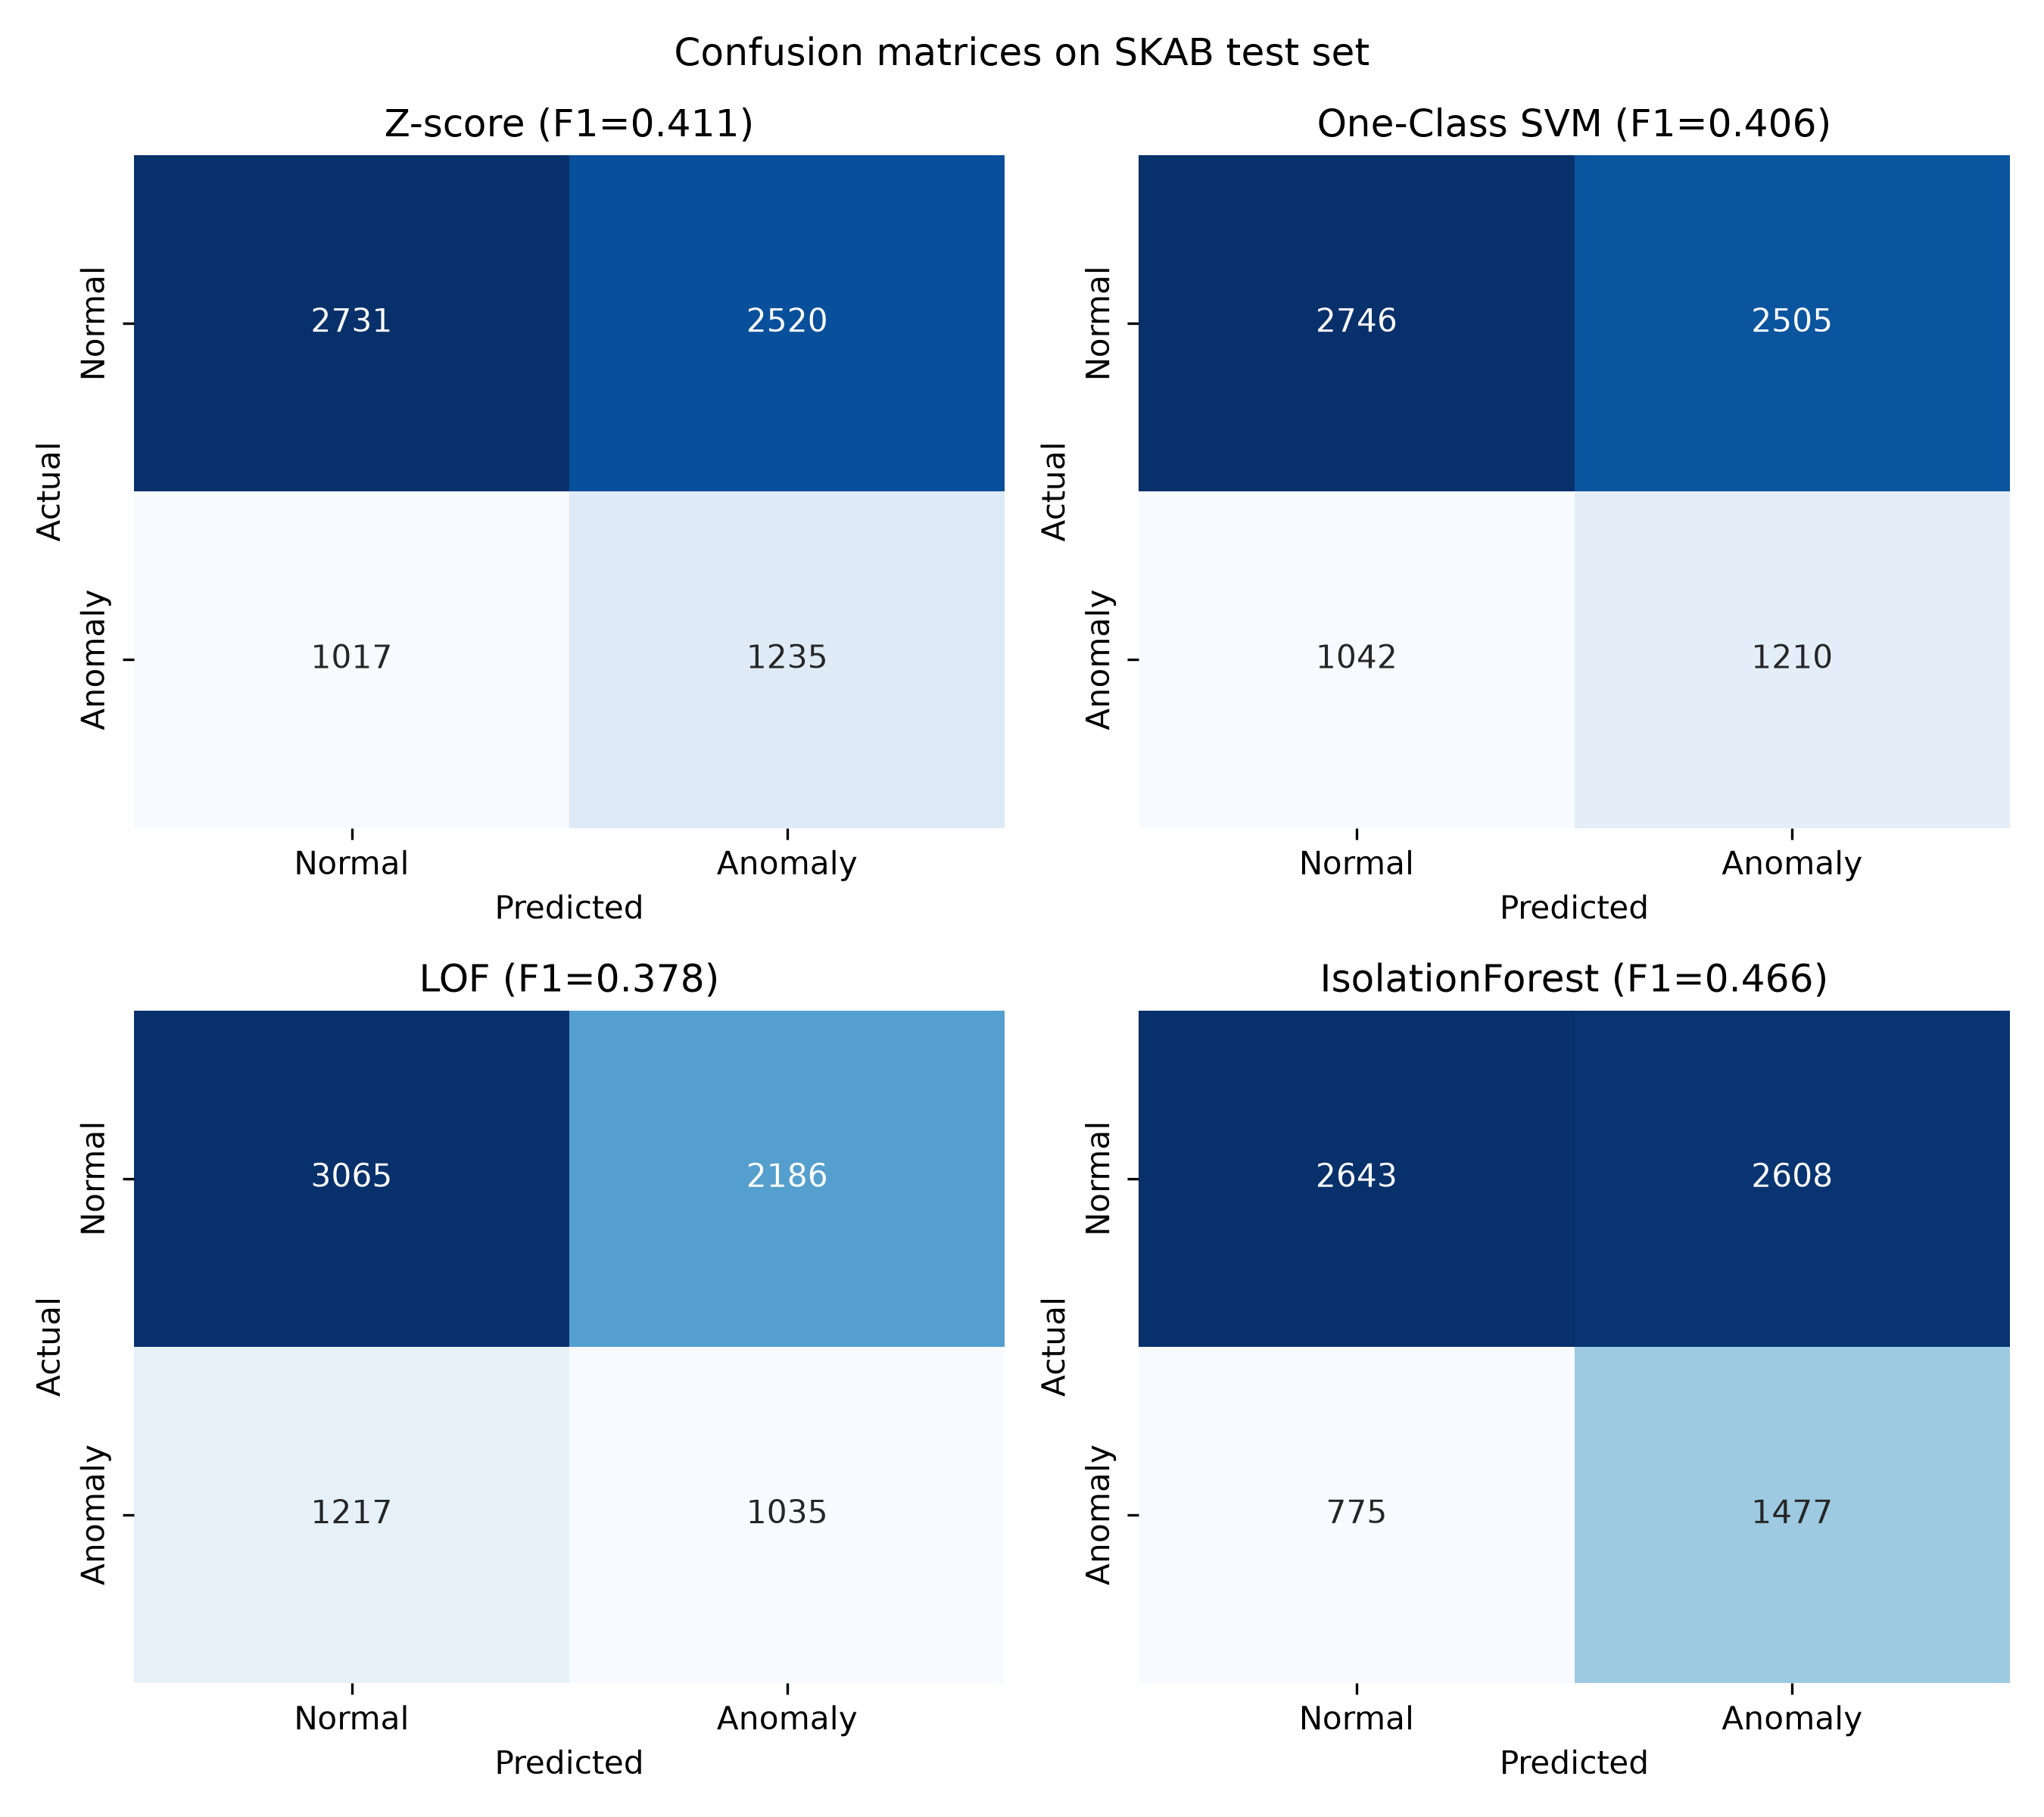
\includegraphics[width=\columnwidth]{confusion_matrices.png}
\caption{Confusion matrices for all six models. Bottom-right cell = faults
correctly caught; bottom-left = faults missed; top-right = false alarms.}
\label{fig:confusion}
\end{figure}

Figure~\ref{fig:timeseries} illustrates Isolation Forest's predictions on a
representative test run, overlaying predicted anomalies on all eight sensor
traces with the true fault intervals shaded. Predicted anomalies align with the
shaded fault regions while a scatter of false alarms appears in nominally normal
stretches---the visual signature of the $0.36$/$0.66$ precision/recall
operating point. Figure~\ref{fig:closeup} zooms to a $\pm 30$\,s window around a
fault onset, where the physical signature of the valve fault (a marked change in
volumetric flow rate at the changepoint) is visible in the raw signal that the
detector responds to.

\begin{figure}[t]
\centering
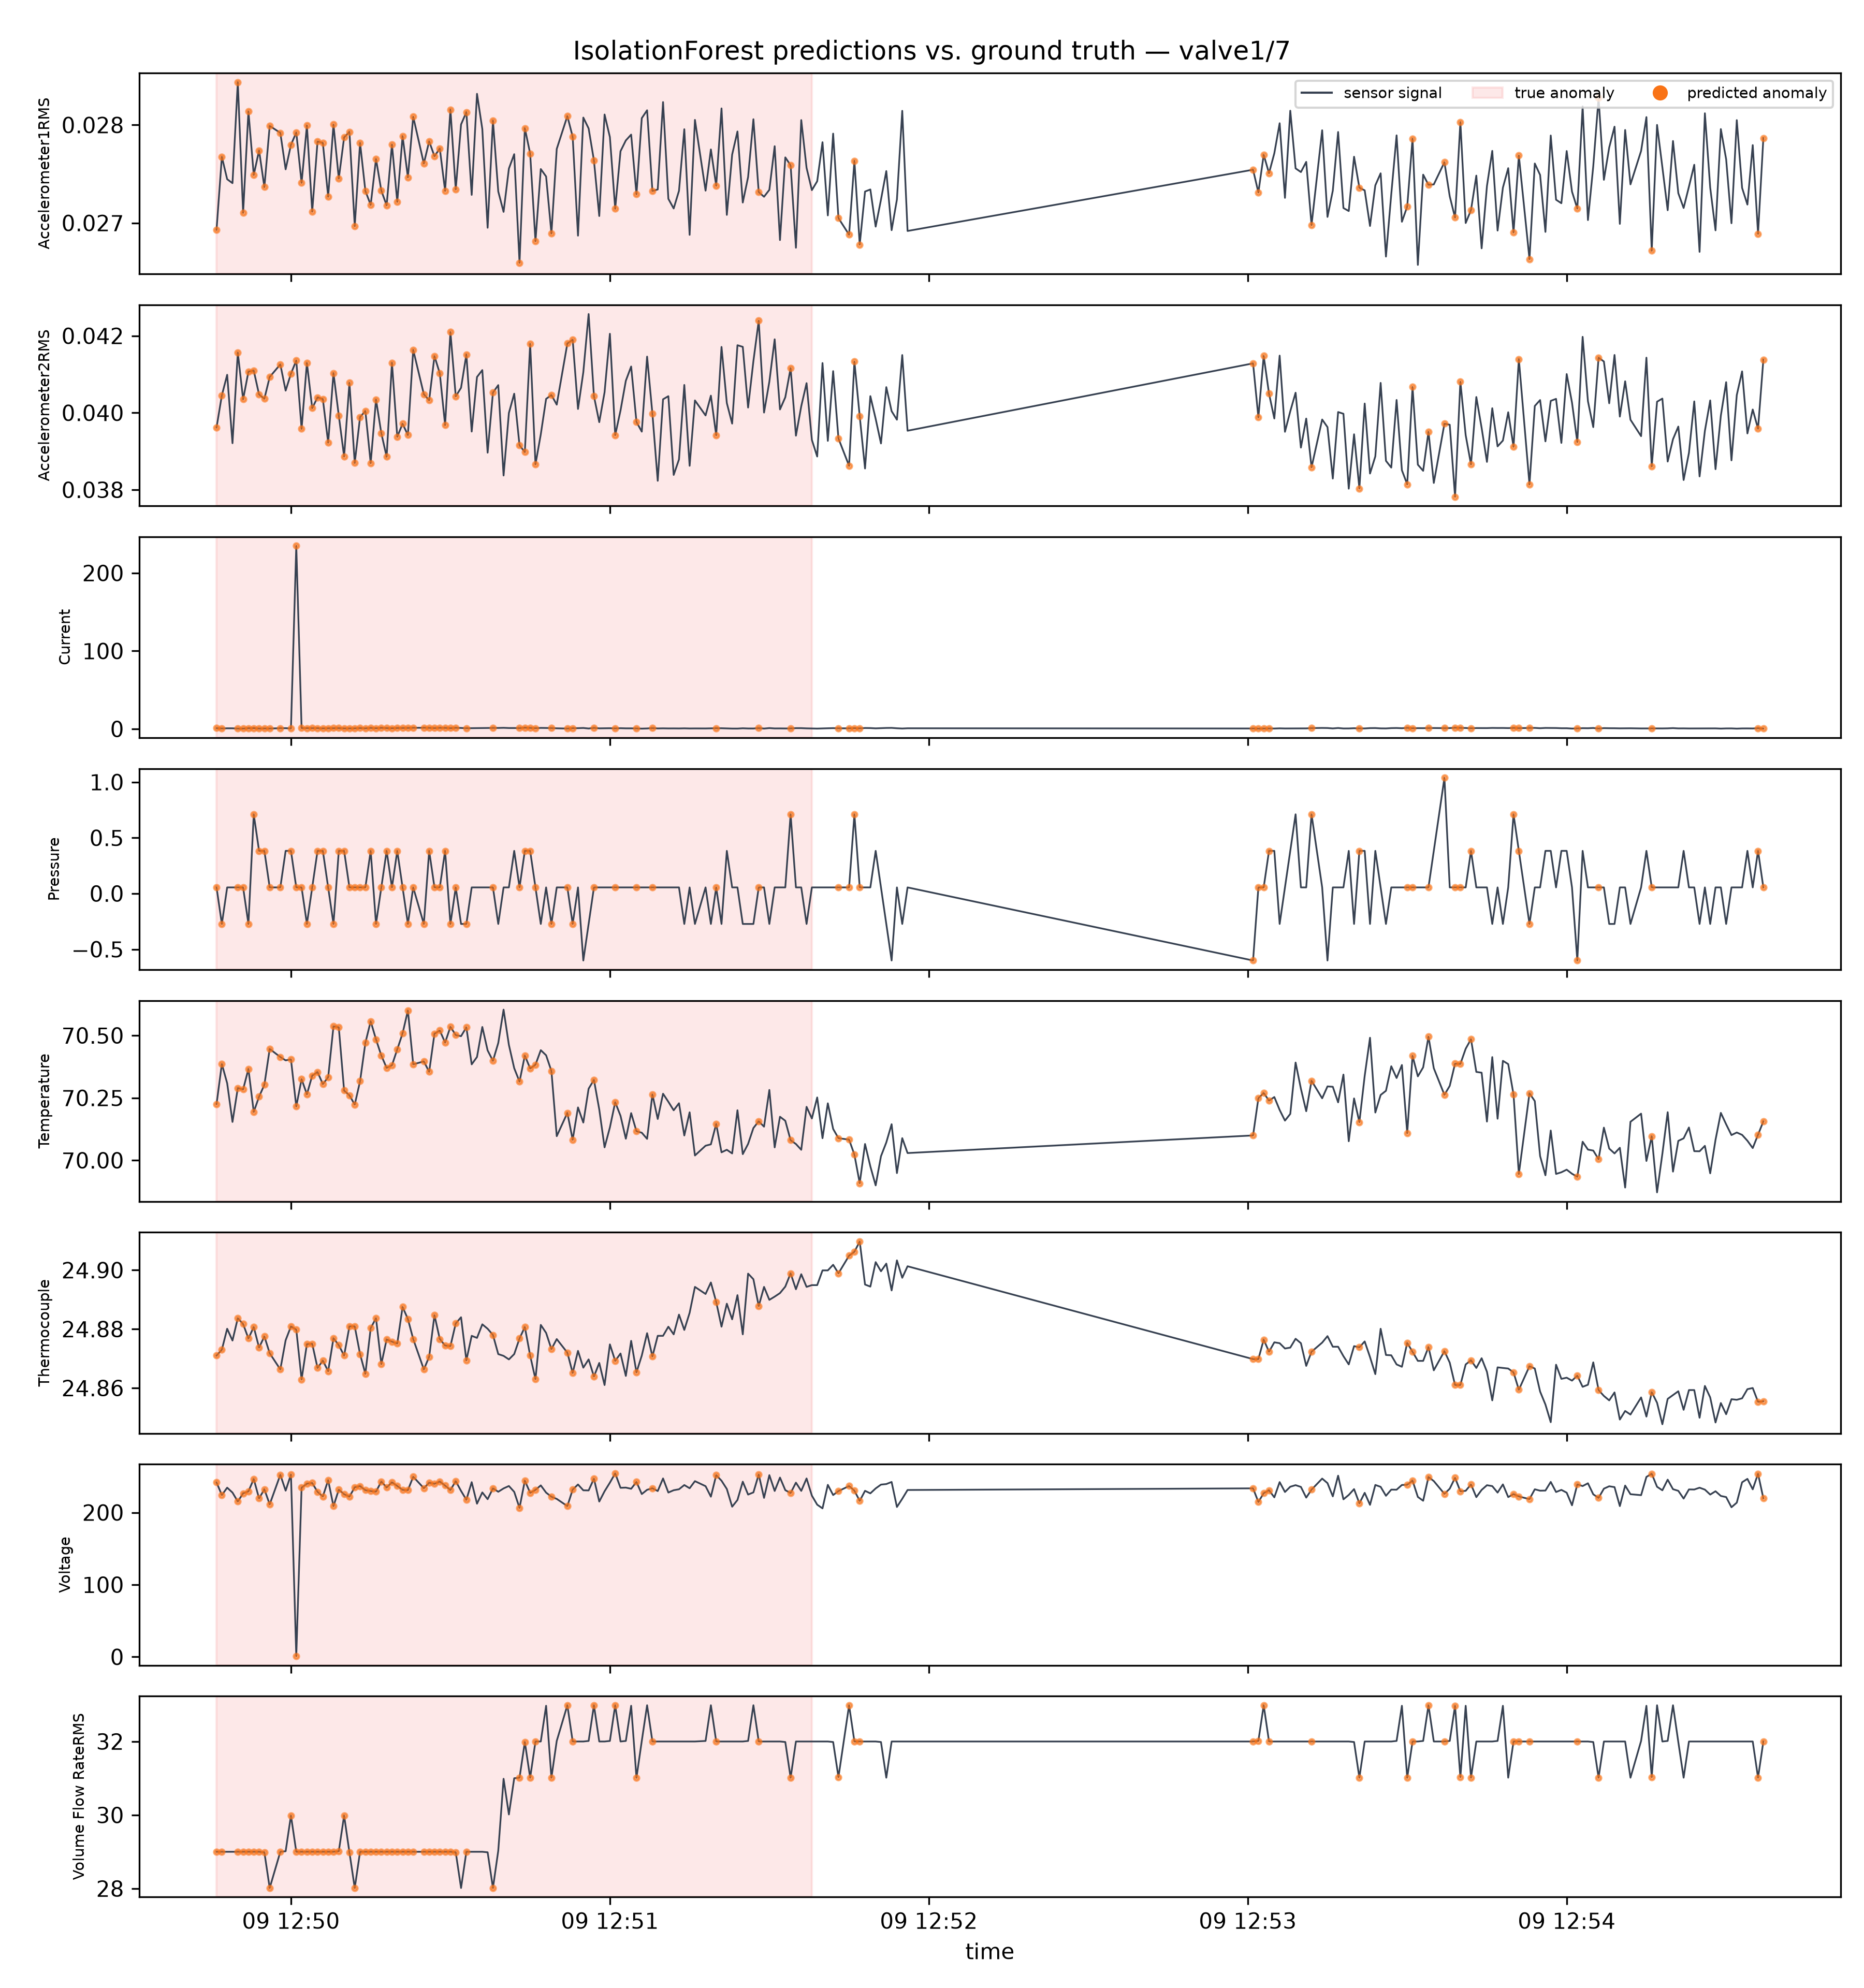
\includegraphics[width=\columnwidth]{timeseries_anomalies.png}
\caption{Isolation Forest predictions on one test run. Red shading = true fault
intervals; markers = predicted anomalies, across all eight sensors.}
\label{fig:timeseries}
\end{figure}

\begin{figure}[t]
\centering
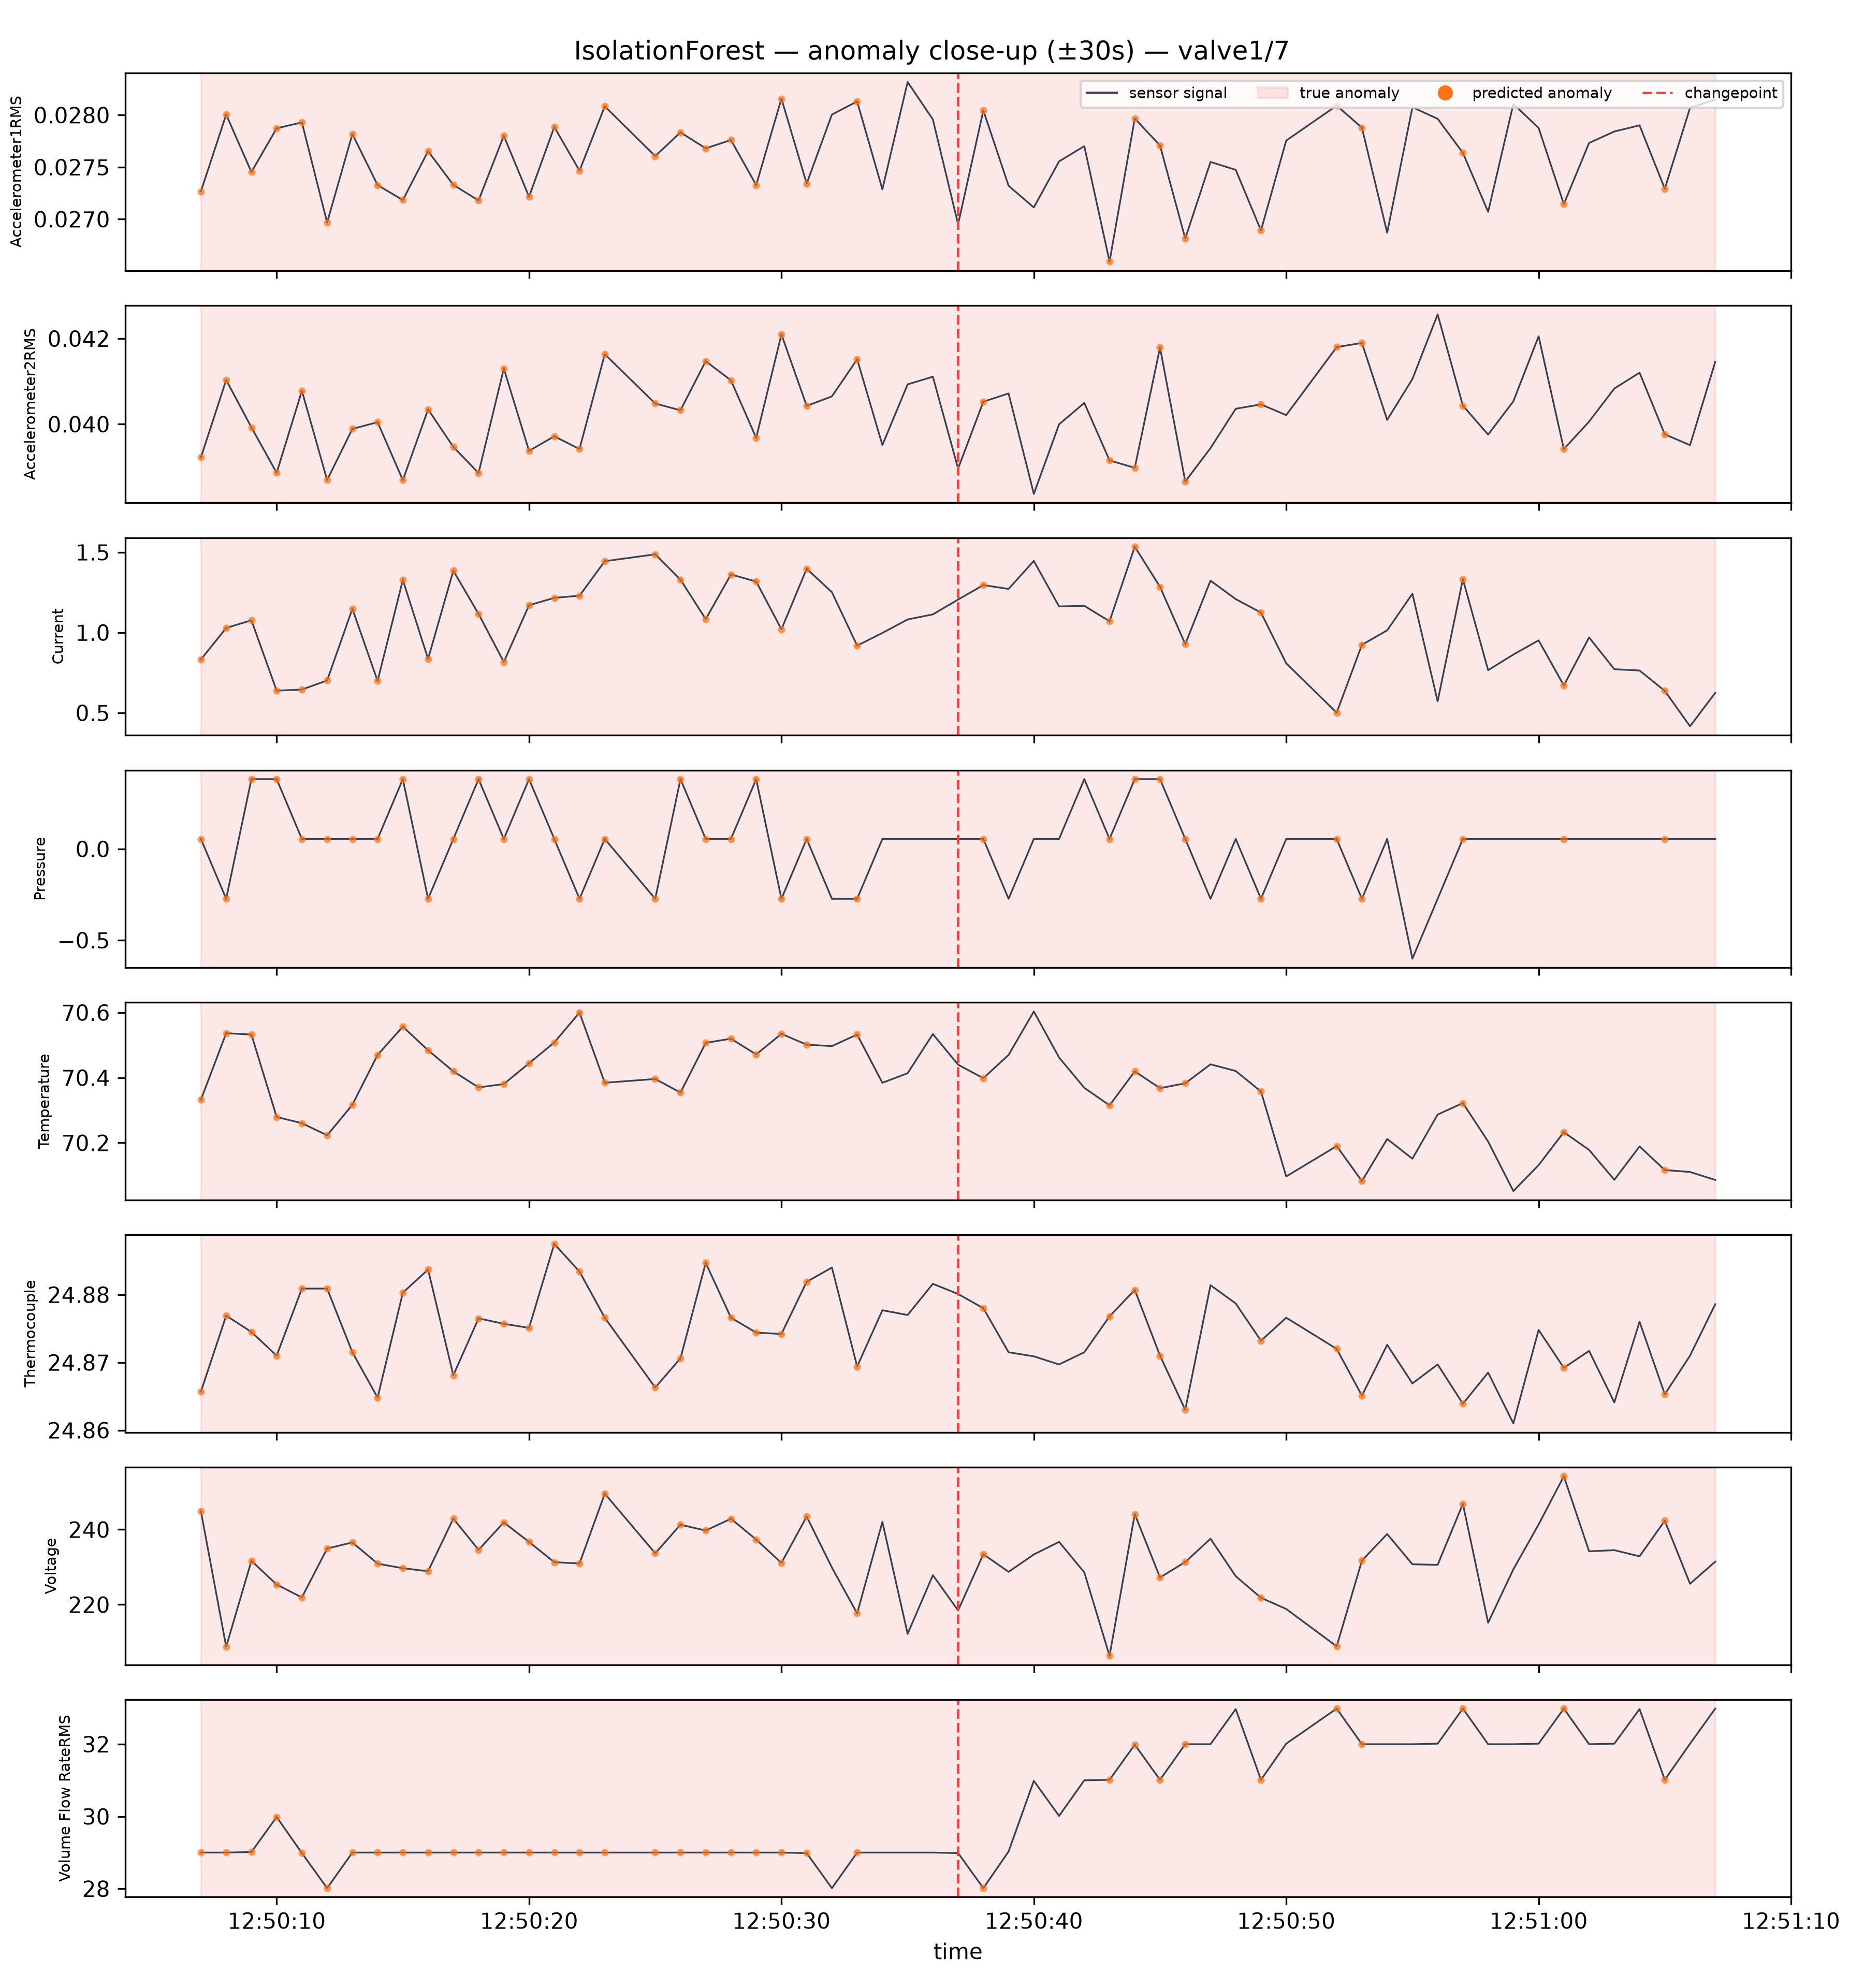
\includegraphics[width=\columnwidth]{anomaly_closeup.png}
\caption{A $\pm 30$\,s close-up around a fault onset (dashed line). The
flow-rate panel shows the physical fault signature the detector reacts to.}
\label{fig:closeup}
\end{figure}

\subsection{Why the Correlation-Based Models Do Not Win}
A notable finding is that the Elliptic Envelope and PCA-reconstruction
detectors---both of which explicitly model inter-sensor \emph{correlation
structure} and are, in principle, well suited to multivariate
faults---do not surpass Isolation Forest. The Elliptic Envelope is the
runner-up (F1 $0.418$) and PCA reconstruction is last (F1 $0.370$). We attribute
this to the representation: our engineered features are short-horizon tabular
statistics, which already expose much of the per-sensor deviation that drives
the labels, while the additional correlation structure these models exploit
provides limited extra signal once the data is in this form. Their theoretical
advantage is most pronounced on \emph{raw sequential} data, which our tabular
pipeline does not hand them. This is an honest negative result and a useful one:
it indicates that, for this feature regime, partition-based isolation is more
effective than covariance or subspace modelling.

\section{Discussion and Limitations}
\label{sec:discussion}
The central result is robust: across six methods and a deliberately conservative
protocol, Isolation Forest is the strongest unsupervised detector on SKAB. We
emphasise, however, several limitations, both to set expectations and to guide
future work.

\textbf{Absolute performance is modest.} The best precision is $\approx 0.36$,
meaning roughly two in three alarms are false. This is characteristic of
unsupervised detection on real industrial data and should temper any claim of
deployment-readiness; the contribution here is a fair \emph{comparison}, not a
state-of-the-art detector. We report these numbers plainly rather than inflating
them through optimistic evaluation tricks.

\textbf{Honesty about leakage.} The headline F1 for Isolation Forest fell from
an earlier $0.496$ to $0.466$ once we removed the leaking wall-clock features.
We retain the lower number because it reflects performance that would transfer
to a genuinely new recording, and we document the episode because such leaks are
common and easy to miss in time-series evaluation.

\textbf{Single dataset, single fault family.} All results are on SKAB, whose
faults are dominated by valve-induced flow restriction. Generalisation to other
machines and fault types (bearing wear, cavitation, electrical faults) is not
established and is left to future work.

\textbf{Tabular features, not sequences.} Our pipeline uses engineered tabular
features rather than raw sequences. Sequence models such as LSTM
encoder--decoders~\cite{malhotra2016} could in principle exploit temporal and
cross-sensor structure that our representation suppresses; the present study
provides the classical baseline against which such models should be measured.

\textbf{Coarse contamination tuning.} The shared contamination value was tuned
on the 43-feature representation prior to the leakage fix; while it is a coarse
knob and our spot checks indicate it remains near-optimal, a full re-tune on the
final 41-feature set is a reasonable refinement.

\section{Conclusion}
\label{sec:conclusion}
We presented a controlled, reproducible comparison of six unsupervised
anomaly-detection models on the real SKAB industrial sensor benchmark, using a
single leakage-free feature representation and a conservative, chronologically
honest evaluation protocol. Isolation Forest emerged as the strongest detector
(F1 $0.466$, recall $0.656$), outperforming distance-, density-, boundary-, and
correlation-based alternatives---including two models that were theoretically
expected to benefit from inter-sensor structure. By reporting modest absolute
scores truthfully and by documenting and removing a wall-clock data leak, we
offer not only a result but a methodological template for trustworthy
unsupervised evaluation on real sensor data. Future work will extend the
comparison to additional datasets and fault families and will benchmark deep
sequence models against the classical baseline established here.

\section*{Reproducibility}
The full pipeline---data loading, feature engineering, all six models,
evaluation, figures, and the trained-model bundle---is implemented in Python
(scikit-learn~\cite{pedregosa2011}) and regenerates every number and figure in
this paper from a single command.

\begin{thebibliography}{00}

\bibitem{skab2020}
I.~D.~Katser and V.~O.~Kozitsin, ``Skoltech Anomaly Benchmark (SKAB),''
Kaggle, 2020. doi: 10.34740/KAGGLE/DSV/1693952.

\bibitem{chandola2009}
V.~Chandola, A.~Banerjee, and V.~Kumar, ``Anomaly detection: A survey,''
\emph{ACM Computing Surveys}, vol.~41, no.~3, pp.~1--58, 2009.

\bibitem{chalapathy2019}
R.~Chalapathy and S.~Chawla, ``Deep learning for anomaly detection: A survey,''
\emph{arXiv preprint arXiv:1901.03407}, 2019.

\bibitem{belay2023}
M.~A.~Belay, S.~S.~Blakseth, A.~Rasheed, and P.~Salvo~Rossi, ``Unsupervised
anomaly detection for IoT-based multivariate time series: Existing solutions,
performance analysis and future directions,'' \emph{Sensors}, vol.~23, no.~5,
art.~2844, 2023.

\bibitem{scholkopf2001}
B.~Sch\"olkopf, J.~C.~Platt, J.~Shawe-Taylor, A.~J.~Smola, and
R.~C.~Williamson, ``Estimating the support of a high-dimensional
distribution,'' \emph{Neural Computation}, vol.~13, no.~7, pp.~1443--1471, 2001.

\bibitem{breunig2000}
M.~M.~Breunig, H.-P.~Kriegel, R.~T.~Ng, and J.~Sander, ``LOF: Identifying
density-based local outliers,'' in \emph{Proc. ACM SIGMOD Int. Conf. Management
of Data}, 2000, pp.~93--104.

\bibitem{liu2008}
F.~T.~Liu, K.~M.~Ting, and Z.-H.~Zhou, ``Isolation forest,'' in \emph{Proc. 8th
IEEE Int. Conf. Data Mining (ICDM)}, 2008, pp.~413--422.

\bibitem{rousseeuw1999}
P.~J.~Rousseeuw and K.~Van~Driessen, ``A fast algorithm for the minimum
covariance determinant estimator,'' \emph{Technometrics}, vol.~41, no.~3,
pp.~212--223, 1999.

\bibitem{shyu2003}
M.-L.~Shyu, S.-C.~Chen, K.~Sarinnapakorn, and L.~Chang, ``A novel anomaly
detection scheme based on principal component classifier,'' in \emph{Proc. IEEE
ICDM Workshop on Foundations and New Directions of Data Mining}, 2003,
pp.~172--179.

\bibitem{malhotra2016}
P.~Malhotra, A.~Ramakrishnan, G.~Anand, L.~Vig, P.~Agarwal, and G.~Shroff,
``LSTM-based encoder-decoder for multi-sensor anomaly detection,'' in
\emph{Proc. ICML Anomaly Detection Workshop}, 2016, arXiv:1607.00148.

\bibitem{rotating2023}
S.~A.~S. \emph{et al.}, ``Machine learning for fault analysis in rotating
machinery: A comprehensive review,'' \emph{Heliyon}, vol.~9, 2023.
% NOTE: confirm exact author list against the published PDF before submission.

\bibitem{pedregosa2011}
F.~Pedregosa \emph{et al.}, ``Scikit-learn: Machine learning in Python,''
\emph{Journal of Machine Learning Research}, vol.~12, pp.~2825--2830, 2011.

\end{thebibliography}

\end{document}
